\documentclass[a4paper,12pt]{article}
\usepackage{graphicx}
\usepackage{amsmath}
\usepackage[margin=1in]{geometry}
\usepackage{amsmath, amssymb}
\usepackage{float}
\usepackage{caption}
\usepackage{subcaption}
\usepackage{xcolor}
\usepackage{fancyhdr}
\usepackage{array}
\usepackage{float}
\usepackage{amsfonts}
\usepackage{graphicx} 
\geometry{a4paper, top=0.7in, left=1in, right=1in, bottom=1in}

\begin{document}
\thispagestyle{fancy}
\fancyhf{} 
\renewcommand{\headrulewidth}{0pt} 

\fancyhead[L]{
        
\includegraphics[width=8cm, height=1.7cm]{comet.jpeg} 
        }
\fancyhead[R]{
    Name: G.MADHU LATHA \\
    Batch:COMET.fwc029 \\
    Date:
}
\vspace{1cm}
\begin{center}
    {\LARGE \textbf{\textcolor{black}{\\  GATE QUESTION \\ EEE 2010 Q52}}}
\end{center}
\vspace{-1cm}
\section*{\textcolor{cyan}{ \\Question :}}
\textbf{The following Karnaugh map represents a function F:} \\
\vspace{1em}
\begin{center}
\begin{minipage}[t]{0.38\textwidth}
\vspace{-3em}
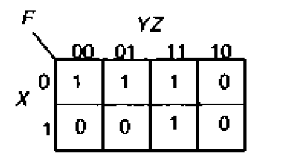
\includegraphics[height=5cm,width=\linewidth]{task31.png}

\end{minipage}
\end{center}
\vspace{0.5cm}
\textbf{Solution for MCQ 1.52}

The given Karnaugh map for the function $F$ is:

\begin{center}
\begin{tabular}{|c|c|>{\centering\arraybackslash}p{0.8cm}|>{\centering\arraybackslash}p{0.8cm}|>{\centering\arraybackslash}p{0.8cm}|>{\centering\arraybackslash}p{0.8cm}|}
\cline{3-6}
\multicolumn{2}{c|}{$F$} & \multicolumn{4}{c|}{$YZ$} \\
\cline{3-6}
\multicolumn{2}{c|}{$X$} & 00 & 01 & 11 & 10 \\
\hline
& 0 & 1 & 1 & 1 & 0 \\
\cline{2-6}
& 1 & 0 & 0 & 1 & 0 \\
\hline
\end{tabular}
\end{center}

To minimize the function $F$, we group the adjacent 1's in the K-map.

\vspace{0.2cm}

\textbf{Step 1: Identify all 1's and their corresponding minterms.}
\begin{itemize}
    \item $X=0, Y=0, Z=0 \implies \overline{X}\overline{Y}\overline{Z}$ (Cell 00)
    \item $X=0, Y=0, Z=1 \implies \overline{X}\overline{Y}Z$ (Cell 01)
    \item $X=0, Y=1, Z=1 \implies \overline{X}YZ$ (Cell 11)
    \item $X=1, Y=1, Z=1 \implies XYZ$ (Cell 11, row 1)
\end{itemize}

\vspace{0.2cm}

\textbf{Step 2: Group the 1's.}

We can form two prime implicants:

\begin{enumerate}
    \item \textbf{Group 1 (Pair):} Group the 1's in cells $(X=0, YZ=00)$ and $(X=0, YZ=01)$.
    \begin{center}
    \begin{tabular}{|c|c|>{\centering\arraybackslash}p{0.8cm}|>{\centering\arraybackslash}p{0.8cm}|>{\centering\arraybackslash}p{0.8cm}|>{\centering\arraybackslash}p{0.8cm}|}
    \cline{3-6}
    \multicolumn{2}{c|}{$F$} & \multicolumn{4}{c|}{$YZ$} \\
    \cline{3-6}
    \multicolumn{2}{c|}{$X$} & 00 & 01 & 11 & 10 \\
    \hline
    & 0 & \fbox{1} & \fbox{1} & 1 & 0 \\
    \cline{2-6}
    & 1 & 0 & 0 & 1 & 0 \\
    \hline
    \end{tabular}
    \end{center}
    This group eliminates $Z$ (since $Z$ changes from 0 to 1 while other variables are constant) and simplifies to $\overline{X}\overline{Y}$.
    
    \item \textbf{Group 2 (Pair):} Group the 1's in cells $(X=0, YZ=11)$ and $(X=1, YZ=11)$.
    \begin{center}
    \begin{tabular}{|c|c|>{\centering\arraybackslash}p{0.8cm}|>{\centering\arraybackslash}p{0.8cm}|>{\centering\arraybackslash}p{0.8cm}|>{\centering\arraybackslash}p{0.8cm}|}
    \cline{3-6}
    \multicolumn{2}{c|}{$F$} & \multicolumn{4}{c|}{$YZ$} \\
    \cline{3-6}
    \multicolumn{2}{c|}{$X$} & 00 & 01 & 11 & 10 \\
    \hline
    & 0 & 1 & 1 & \fbox{1} & 0 \\
    \cline{2-6}
    & 1 & 0 & 0 & \fbox{1} & 0 \\
    \hline
    \end{tabular}
    \end{center}
    This group eliminates $X$ (since $X$ changes from 0 to 1 while other variables are constant) and simplifies to $YZ$.
\end{enumerate}

\vspace{0.2cm}

\textbf{Step 3: Write the minimized Boolean expression.}
The minimized form of the function $F$ is the sum of these prime implicants:
$$ F = \overline{X}\overline{Y} + YZ $$

Comparing this with the given options:
(A) $F = \overline{X}\overline{Y} + YZ$
(B) $F = \overline{X}\overline{Y} + YZ$
(C) $F = \overline{X}\overline{Y} + Y\overline{Z}$
(D) $F = \overline{X}\overline{Y} + Y\overline{Z}$

Both options (A) and (B) match our derived minimized expression. Assuming only one is the correct option in a multiple-choice setting, if there were a distinction between (A) and (B) in the original problem format, one would be chosen. Based on the image provided, (B) is indicated as the correct option.

The final answer is $\boxed{F = \overline{X}\overline{Y} + YZ}$.
\end{document}
